% vim: set spelllang=fr foldmethod=marker:
\section{Simulation du processus}\label{se:sec:simul}

Le processus de sélection des \cns selon leur énergie résiduelle a lui aussi conduit à la réalisation de plusieurs simulations, afin de le comparer au modèle de sélection pseudo-aléatoire.
Le logiciel \nsiii a été utilisé pour l'occasion.

Nous avons exécuté plusieurs instances de simulation en nous concentrant sur la consommation en énergie ainsi que sur la répartition de la charge dans le cluster.
\todo{link to detection results~\cite{GMT12, BMM13}}
Les paramètres utilisés lors des simulations sont présentés en \tabref{se:table:parameters}.


We launched several simulation instances and chose to focus on the energy consumption and load balancing in the cluster.
To obtain data about detection rate or false positive values of the \cns scheme, the reader is redirected to our previous work\cite{GMT12, BMM13}.
When we implemented our solution, we set the parameters of the simulation as detailed in Table~\ref{se:table:parameters}.

\begin{table}[ht]
    \centering
    \caption{Paramètres utilisés pour les simulations}
    \medskip
    \begin{tabular}{l l}
        \toprule
        Paramètre                          & Valeur\\
        \midrule
        Nombre de nœuds                    & 30 (plus 1~\CH)\\
        Nombre de \cns                     & 4\\
        Probabilité de sélection d'un \vns & 33~\%\\
        Période de renouvellement des \cns & 1~minute\\
        Durée totale de simulation         & 30~minutes\\
        Forme du cluster                   & carré\\
        Taille du cluster                  & 2$\times$50~mètres de diagonale\\
        Portée de transmission             & 50~mètres\\
        Position des nœuds                 & \CH: au centre; autres: aléatoire\\
        Mobilité des nœuds                 & nulle\\
        Débit d'émission des nœuds normaux & 1024~octets toutes les 3~secondes\\
        Requêtes des \vns (par \cn cible)  & 1024~octets toutes les 5~secondes\\
        \bottomrule
    \end{tabular}\label{se:table:parameters}
\end{table}

Ces simulations ont permis d'obtenir l'énergie résiduelle de chaque capteur à intervalles réguliers (une minute).
À partir de ces données, nous avons pu retracer les courbes d'évolution de la moyenne et de l'écart-type de la distribution de l'énergie résiduelle entre les nœuds.
L'énergie résiduelle du \ch a été volontairement ignorée.
\begin{figure}[ht]
    \centering
    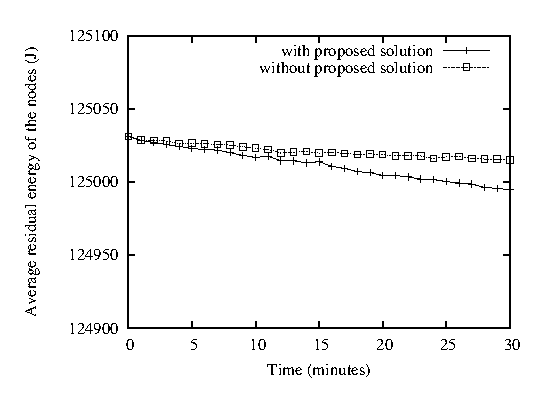
\includegraphics[width=.96\linewidth]{\chapterfig/mean.eps}
    \caption{Valeur moyenne de l'énergie des nœuds (à l'exception du \ch) en fonction du temps}\label{se:fig:mean}
\end{figure}
La valeur moyenne est présentée sur la \figref{se:fig:mean}.
L'augmentation des valeurs à $t=11$~minutes ainsi qu'à $t=15$~minutes sur la courbe de la sélection par l'énergie provient de l'effet de récupération des batteries.
Ces résultats sont conformes aux attentes: le processus de sélection par l'énergie consomme davantage d'énergie dans le réseau, ce que l'on peut imputer au rôle supplémentaire de \vn mis en place.
Étant donné que les \vns vont avoir à sortir périodiquement de leur état de veille pour envoyer une requête au \cn surveillé, écouter la réponse, et calculer une consommation théorique, le besoin en ressources énergétiques se retrouve logiquement affecté par rapport au processus de sélection pseudo-aléatoire.

Les données de contrôle des deux méthodes proposées apparaissent sur la \figref{se:fig:overhead}.
\begin{figure}[ht]
    \centering
    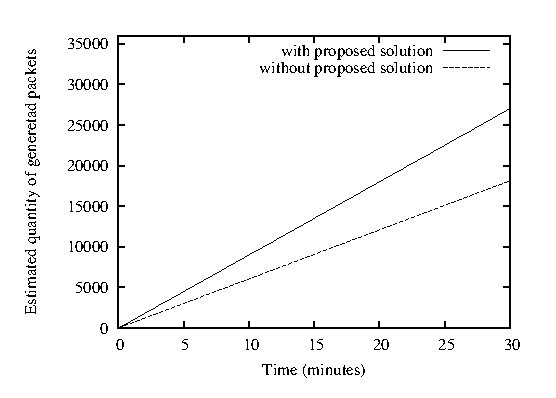
\includegraphics[width=.96\linewidth]{\chapterfig/overhead.eps}
    \caption{Estimation du nombre total de paquets générés au cours de la simulation au cours du temps}\label{se:fig:overhead}
\end{figure}
Ici encore, l'usage des \vns entraîne une augmentation des ressources consommées; il faut également tenir compte des messages (moins nombreux) envoyés par chaque capteur au moment du renouvellement de la sélection.

L'écart-type de la distribution en énergie résiduelle des nœuds est présenté sur la \figref{se:fig:stddev}.
\begin{figure}[ht]
    \centering
    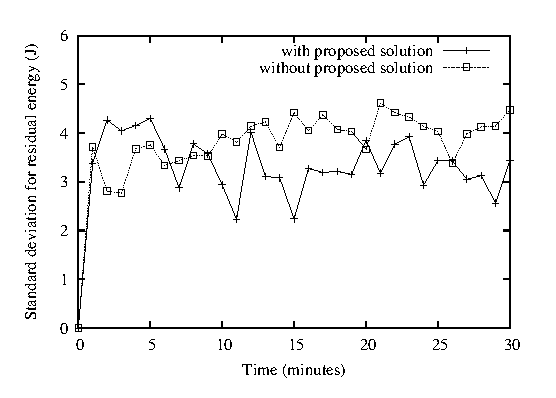
\includegraphics[width=.96\linewidth]{\chapterfig/stddev.eps}
    \caption{Écart-type pour l'énergie résiduelle des nœuds (à l'exception du \ch) au cours du temps}\label{se:fig:stddev}
\end{figure}
Durant les premières minutes de la simulation, la sélection par l'énergie crée une dispersion plus affirmée de la charge en énergie du réseau, à cause des \vns (il y a davantage de capteurs qui endossent des rôles consommant plus d'énergie).
Mais après les sept premières minutes environ, l'écart-type pour le processus de sélection par l'énergie devient et demeure inférieur à celui associé à la méthode pseudo-aléatoire.
Cela traduit la meilleure répartition de la charge énergétique dans le cluster, ce qui était l'objectif de cette solution.
La différence entre les écart-types des deux méthodes est malgré tout peu élevé: cela tient entre autres aux modèles implémentés pour les simulations.
Comme nous disposons d'un générateur de nombres pseudo-aléatoires efficace, à partir d'un certain nombre de renouvellements de la sélection, tous les capteurs vont endosser le rôle de \cn à peu près le même nombre de fois si la sélection se fait de façon pseudo-aléatoire.
Et comme les capteurs ont également des activités de mesure identique, cette méthode (pseudo-aléatoire) fournit, dans notre cas, une excellente répartition de la charge dans le cluster.
Dans une situation où les capteurs auraient des niveaux d'activité différents ---~si par exemple un évènement à détecter se produit beaucoup plus souvent dans une certaine région géographique du cluster~--- alors la consommation, avec cette méthode, ne serait plus nécessairement équilibrée entre tous les nœuds du cluster.
Tandis que la sélection des \cns par l'énergie permettrait de rétablir cet équilibre.
